\subsection{Einf\"uhrung}
Der Vergleich zweier mit einer Rangfolge versehenen Listen ist ein bekanntes Problem. In unserem Fall handelt es sich um den spezialfall von Listen gleicher und fester L\"ange, aber einer potentiell unendlichen Zahl verschiedener W\"orter. Desweiteren sind die Listen nicht \emph{Conjoint}, was bedeutet, dass nicht nur gemeinsame W\"orter in den verschiedenen Listen auftauchen. In \cite{webber2010similarity} werden als Einleitung f\"ur ein Ma\ss, dass in der Lage ist auch unendliche Listen und Listen verschiedener L\"ange vergleichen zu k\"onnen geeignete Verfahren vorgestellt um solche Listen zu vergleichen. Das gew\"ahlte Verfahren \emph{Average Overlap} wird von den Autoren als \emph{top-k ranking} identifiziert. Also ein Ranking bis zu einer definierten Tiefe von k.\\
Der Vorteil des genutzten Verfahrens f\"ur unseren Anwendungsfall ist, dass der Rang der W\"orter einen Einfluss auf das Ma\ss haben. \"Ahnlichkeiten an der Spitze der Liste werden st\"arker gewichtet.\\
Das Verfahren ist ein Mengenbasierter Ansatz. Listen sind sich dann \"ahnlich, wenn sie die relative Anzahl gemeinsamer W\"orter hoch ist. Um nun aufsteigende Gewichtungen zu erhalten wird nun nicht nur die gesamte \"Uberlappung zweier Listen gemessen, sondern die Listen in K Listen unterteilt, wobei K die L\"ange der Listen ist und jede einzelne Liste jeweils alle Elemente bis zu dem Rang des Laufindexes k von 1 bis K enth\"alt. Also eine Liste der Form: [[ Wort 1],[Wort 1, Wort 2], ...]. Nun wird bei den einzelnen Listen gleicher L\"ange die relative \"Uberlappung gemessen. Um nun das Verlgleichsma\ss  zu erhalten wird der Durchschnitt aller errechneten Werte gemessen.  Formalisiert ergibt dies:
\begin{equation}
AO(S,T) = \frac{\sum_{k=1}^K\frac{| M(S_k) \cap M(T_k)|}{k}}{K}
\end{equation}
Wobei $S$ und $T$ zwei Listen sind, der tiefgestellte Index $k$ die Teilliste bis zum Rang $k$ angibt und $K$ die L\"ange der beiden Listen definiert. $M$ ist hierbei die Abbildung einer Liste auf die Menge der enthaltenen Elemente.\\
%Beispiel:\\
\subsection{Ergebnisse}
Hier die Ergebnisse f\"ur den 1.5.2015 mit der Listenl\"ange $K=1000$
\begin{table}[ht]
\centering
\begin{tabular}{rllr}
  \hline
 & List & List\_to\_compare & average\_overlap \\ 
  \hline
1 & tf\_idf & poisson & 0.66 \\ 
  2 & tf\_idf & z-score & 0.18 \\ 
  3 & tf\_idf & freqratio & 0.31 \\ 
  4 & tf\_idf & freqratio\_old & 0.31 \\ 
  5 & tf\_idf & poisson\_old & 0.66 \\ 
  6 & poisson & z-score & 0.15 \\ 
  7 & poisson & freqratio & 0.16 \\ 
  8 & poisson & freqratio\_old & 0.16 \\ 
  9 & poisson & poisson\_old & 1.00 \\ 
  10 & z-score & freqratio & 0.16 \\ 
  11 & z-score & freqratio\_old & 0.16 \\ 
  12 & z-score & poisson\_old & 0.15 \\ 
  13 & freqratio & freqratio\_old & 1.00 \\ 
  14 & freqratio & poisson\_old & 0.16 \\ 
  15 & freqratio\_old & poisson\_old & 0.16 \\ 
   \hline
\end{tabular}
\caption{Avarage Overlap Comparison} 
\label{AvarageOverlapComparison}
\end{table}\begin{figure}[htbp] 
  \centering
     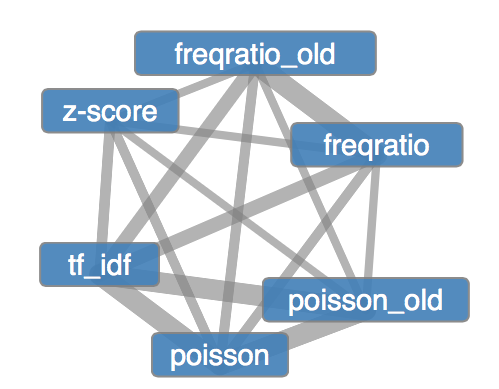
\includegraphics[width=0.7\textwidth]{pictures/comparison.png}
  \caption{Graph of Average Overlap}
  \label{fig:comparisonGraph}
\end{figure}
